\section{Materiales y métodos}

En esta sección serán expuestos las diferentes herramientas y métodos utilizados para llevar a cabo el proyecto, así como los resultados obtenidos con cada una de ellas.

\subsection{Human Phenotype Ontology}

La \textbf{Human Phenotype Ontology (HPO)} es un proyecto que desarrolla un vocabulario estandarizado y jerárquico para describir fenotipos humanos, con el objetivo de apoyar el diagnóstico y la investigación de enfermedades genéticas. Además de definir y organizar características fenotípicas específicas, la HPO permite identificar los genes y variantes genéticas asociadas a cada fenotipo, de esta manera facilita el análisis de correlaciones genotipo-fenotipo a los usuarios.

Para realizar este estudio, el primer pasó que se llevó a cabo fue la obtención de los genes relacionados con el fenotipo. Los descargamos de la página Human Phenotype Ontology mediante la introducción del ID del fenotipo, en nuestro caso "HP:0000526". Una vez obtenidos los genes, realizamos una red de interacción de los genes asociados a nuestro fenotipo mediante la herramienta STRINGDB.
 

\subsection{STRING}


STRING es una base de datos que permite analizar y visualizar interacciones entre proteínas y genes. A continuación, se muestras los pasos llevados a cabo para obtener una red de interacción de los genes de un fenotipo concreto:

\begin{itemize}
	\item Visitamos la página de STRING
	\item Seleccionamos la opción para intnroducir multiples proteínas
	\item Introducimos solo los nombres de los genes descargados de Human Phenotype Ontology.
	\item Especificamos la especie, en este caso, Homo sapiens.
	\item STRING generará una red de interacciones, mostrando conexiones basadas en interacciones experimentales, predicciones y bases de datos de coexpresión.
	\item Se guarda como imagen la red obtenida.
\end{itemize}

Entre los objetivos del uso de STRING están visualizar las interacciones proteicas conocidas y predichas, identificar posibles proteínas clave o "hubs" dentro de la red y evaluar la conectividad y la funcionalidad de los genes en el contexto del fenotipo elegido.
	
Tras introducir el nombre de todos los genes asociados a nuestro fenotipo obtuvimos la siguiente red de interacciones:

\newpage

\begin{figure}[h] % [h] indica que queremos la imagen aquí, en la posición actual
	\centering
	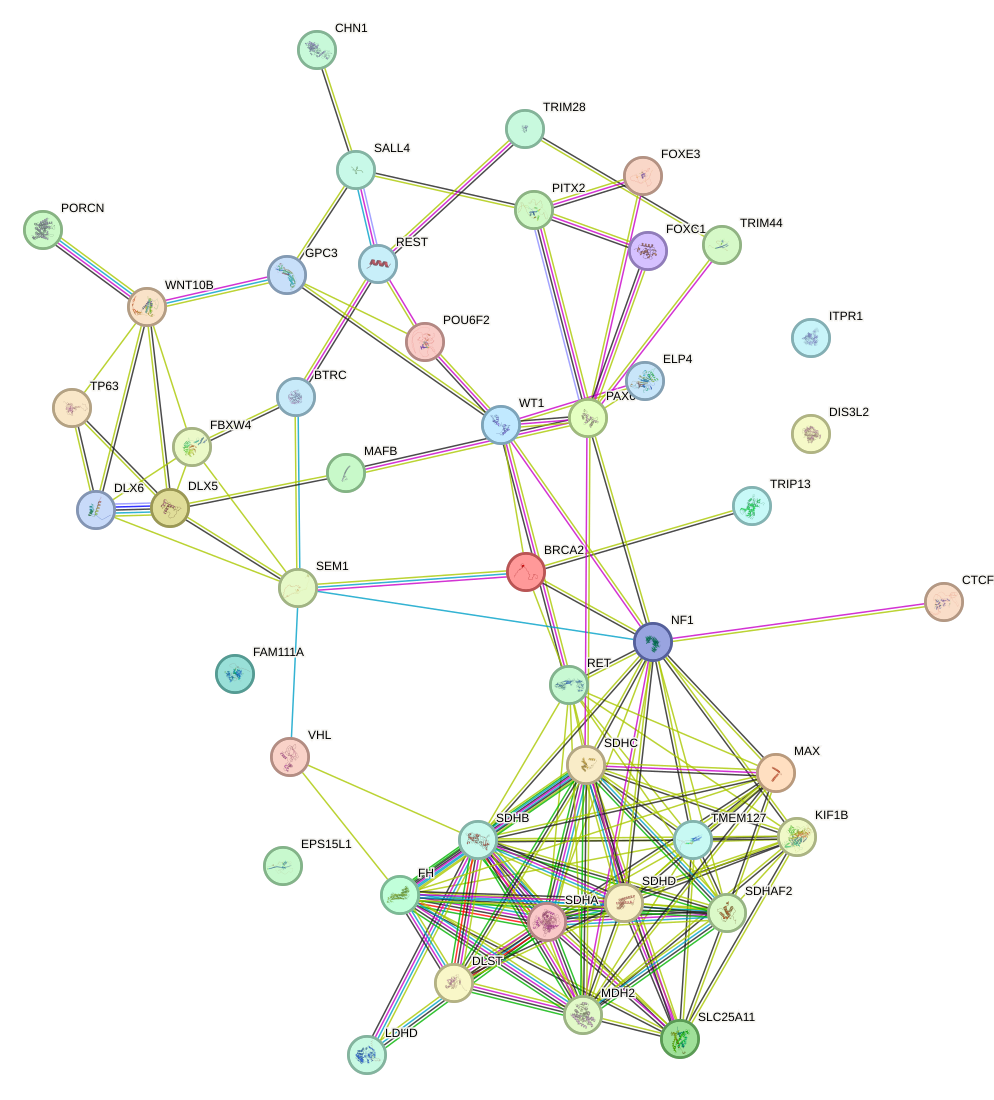
\includegraphics[width=1\textwidth]{figures/red_interaccion_aniridia.png} % Especifica la ruta y el tamaño
	\caption{Red de interacción con los genes asociados al fenotipo HP:0000526} % Agrega una leyenda si deseas
	\label{fig:mi-imagen} % Etiqueta para referenciar la imagen en el texto
\end{figure}

\subsection{Python}
Python es uno de los lenguajes de programación más usados del mundo. Se trata de un lenguaje de alto nivel con una sintaxis sencilla y fácil de entender que dispone de multitud de paquetes de código abierto. Se caracteriza por ser interpretado, es decir, no se requiere de compilación previa a instrucciones de lenguaje máquina ya que se emplea un entorno o intérprete para ejecutar el código.
La versión utilizada en este proyecto es ?.

\subsection{R}
R es otro de los lenguajes de programación más importantes en el campo de la estadística. Es un entorno de software libre y también es un lenguaje interpretado. A diferencia de otros softwares de análisis de datos, R tiene un entorno completamente integrado y coherente. Proporciona una amplia gama de técnicas estadísticas y gráficas. La versión utilizada en este proyecto es ?.

\subsection{iGraph}
iGraph es una biblioteca de código abierto utilizada para el análisis y visualización de redes complejas. Es una herramienta muy útil para el estudio de los sistemas biológicos ya que estos están compuestos por genes, moléculas, proteínas, etc, que interactúan formando grafos complejos de analizar a simple vista. Está implementado en C, aunque también puede ser utilizado en otros lenguajes como R y Python. 

Esta herramienta presenta muchas ventajas, entre las que destacamos: la integración de todo tipo de datos ómicos, la visualización de datos de forma interactiva, mejora la comprensión de las relaciones entre las distintas biomoléculas del sistema, permite la identificación de nodos clave en la red biológica, facilita el descubrimiento de grupos funcionales de genes o proteínas y predice cómo ciertas modificaciones podrían perturbar los sistemas.

\subsection{Pandas}
Pandas se trata de una popular librería de Python de código abierto muy necesaria para el ámbito de Data Science y Machine Learning. Proporciona unas estructuras poderosas y flexibles implementando todas las herramientas necesarias para el análisis de datos, ya que permite la carga, modelado, análisis, manipulación y preparación de datos.

\subsection{Algoritmos de clusterización}
En el presente proyecto, uno de los objetivos es la identificación de patrones entre los distintos genes asociados al fenotipo de la aniridia. Para ello, es necesario el agrupamiento de aquellas biomoléculas con mayor similitud dentro nuestra red biológica, así que se aplicarán algoritmos nos permitan detectar estructuras sin necesidad de tener conocimiento previo. Vamos a hablar de los algoritmos de Givan-Newman, de optimización voraz, de propagación de etiquetas y de Louvain.

Primero, tenemos el algoritmo de Givan-Newman, que es uno de los métodos más utilizados para la detección de comunidades dentro de sistemas complejos de datos. Su funcionamiento se basa en eliminar progresivamente aquellos enlaces que conectan grupos de nodos con mayor densidad dentro de la red, para visualizar finalmente subgrafos desconectados que representan las comunidades.

Por otra parte, el algoritmo de optimización voraz es un algoritmo que dado un problema, elige aquellas decisiones localmente óptimas con el propósito de encontrar la solución más óptima globalmente. A medida que va tomando unas decisiones, el algoritmo no reconsidera ningún paso ya realizado.

Además, el algoritmo de propagación de etiquetas es una técnica que nos permite encontrar comunidades dentro del sistema velozmente. El funcionamiento se basa en la asignación de etiquetas a nodos, que en cada iteración se van propagando por la red y converge finalmente cuando cada nodo posee la etiqueta perteceneciente a su vecino más cercano. Una de las ventajas de este algoritmo es que no es necesaria la predefinición de un número de clústers.

Por último, el algoritmo de Louvain se basa en el concepto de modularidad, es decir, tiene como objetivo maximizar el número de aristas dentro de una comunidad y minimizar el número de relaciones entre distintas comunidades. Este algoritmo es muy recomendable para sistemas biológicos muy amplios, ya que se obtienen comunidades compactas y bien definidas.

\subsection{Otras librerías empleadas}

\subsection{Software empleado para la generación de diagramas}

\subsection{GitHub?}

\subsection{Flujo de trabajo}
